\documentclass{beamer}
%\documentclass[handout]{beamer}
\usepackage{amsmath,amsfonts,amssymb}
\usepackage{beamerthemeshadow}
\usepackage{array}
\usepackage{pgf,pgfarrows,pgfnodes,pgfautomata,pgfheaps,pgfshade}
\usepackage[utf8]{inputenc}
\usepackage{colortbl}
\usepackage{pdfpages}
\usepackage{xcolor}
\usepackage{adjustbox}
\usepackage{tabularx}
\def\tabularxcolumn#1{m{#1}}
%%Check if we are compiling under latex or pdflatex
% \ifx\pdftexversion\undefined
%   \usepackage[dvips]{graphicx}
%\else
%   \usepackage[pdftex]{graphicx}
%\fi

\usepackage{pythontex}
%\beamertemplatetransparentcovereddynamic
% This is the file main.tex
\mode<presentation>
{\usetheme{Berlin} }

%% \AtBeginSection[]
%% {
%%    \begin{frame}
%%        \frametitle{Guión}
%%        \tableofcontents[currentsection]
%%    \end{frame}
%% }

\graphicspath{{../figures/}}


\newcommand{\field}[1]{\mathbb{#1}}
\newcommand{\E}{\field{E}}
\newcommand{\R}{\field{R}}
\newcommand{\N}{\field{N}}
\newcommand{\Z}{\field{Z}}
\newcommand{\Q}{\field{Q}}
\newcommand{\EE}{\field{E}}
\newcommand{\FF}{\field{F}}
\newcommand{\GG}{\field{G}}
\renewcommand{\L}{\field{L}}
\renewcommand{\P}{\field{P}}
\newcommand{\LL}{{\mathfrak L}}

\renewcommand{\arraystretch}{1.5}
\hypersetup{
   pdfpagemode={FullScreen},
   pdftitle = {},
   pdfauthor={Mathieu Kessler},
colorlinks=true,linkcolor=red
}

\title{Regularización para regresión y clasificación }
\author[Kessler]{Mathieu Kessler}
\institute[UPCT]{
  Departamento de Matemática Aplicada y Estadística\\
  Universidad Politécnica de Cartagena}

\date[Cartagena]{Cartagena}

\begin{document}

\begin{frame}
  \titlepage
\end{frame}
 \begin{frame}\frametitle{El problema del sobreajuste}
      \begin{itemize}
     \item<+-> Si añadimos características adicionales (por ejemplo potencias de las características) podemos a veces  mejorar el ajuste a nuestro conjunto de entrenamiento, o mejorar nuestra capacidad de clasificar sus observaciones.
     \item<+-> Pero, puede ser que la mejora de este ajuste sea artificial
     \item<+> Hemos mejorado aparentemente el ajuste para el conjunto de entrenamiento pero puede empeorar en el conjunto de test.
       
     \end{itemize}
 \end{frame}
 \begin{frame}\frametitle{Ejemplo: Ajuste con una característica $x$}
   \begin{overlayarea}{\textwidth}{8cm} 
 \begin{center}
   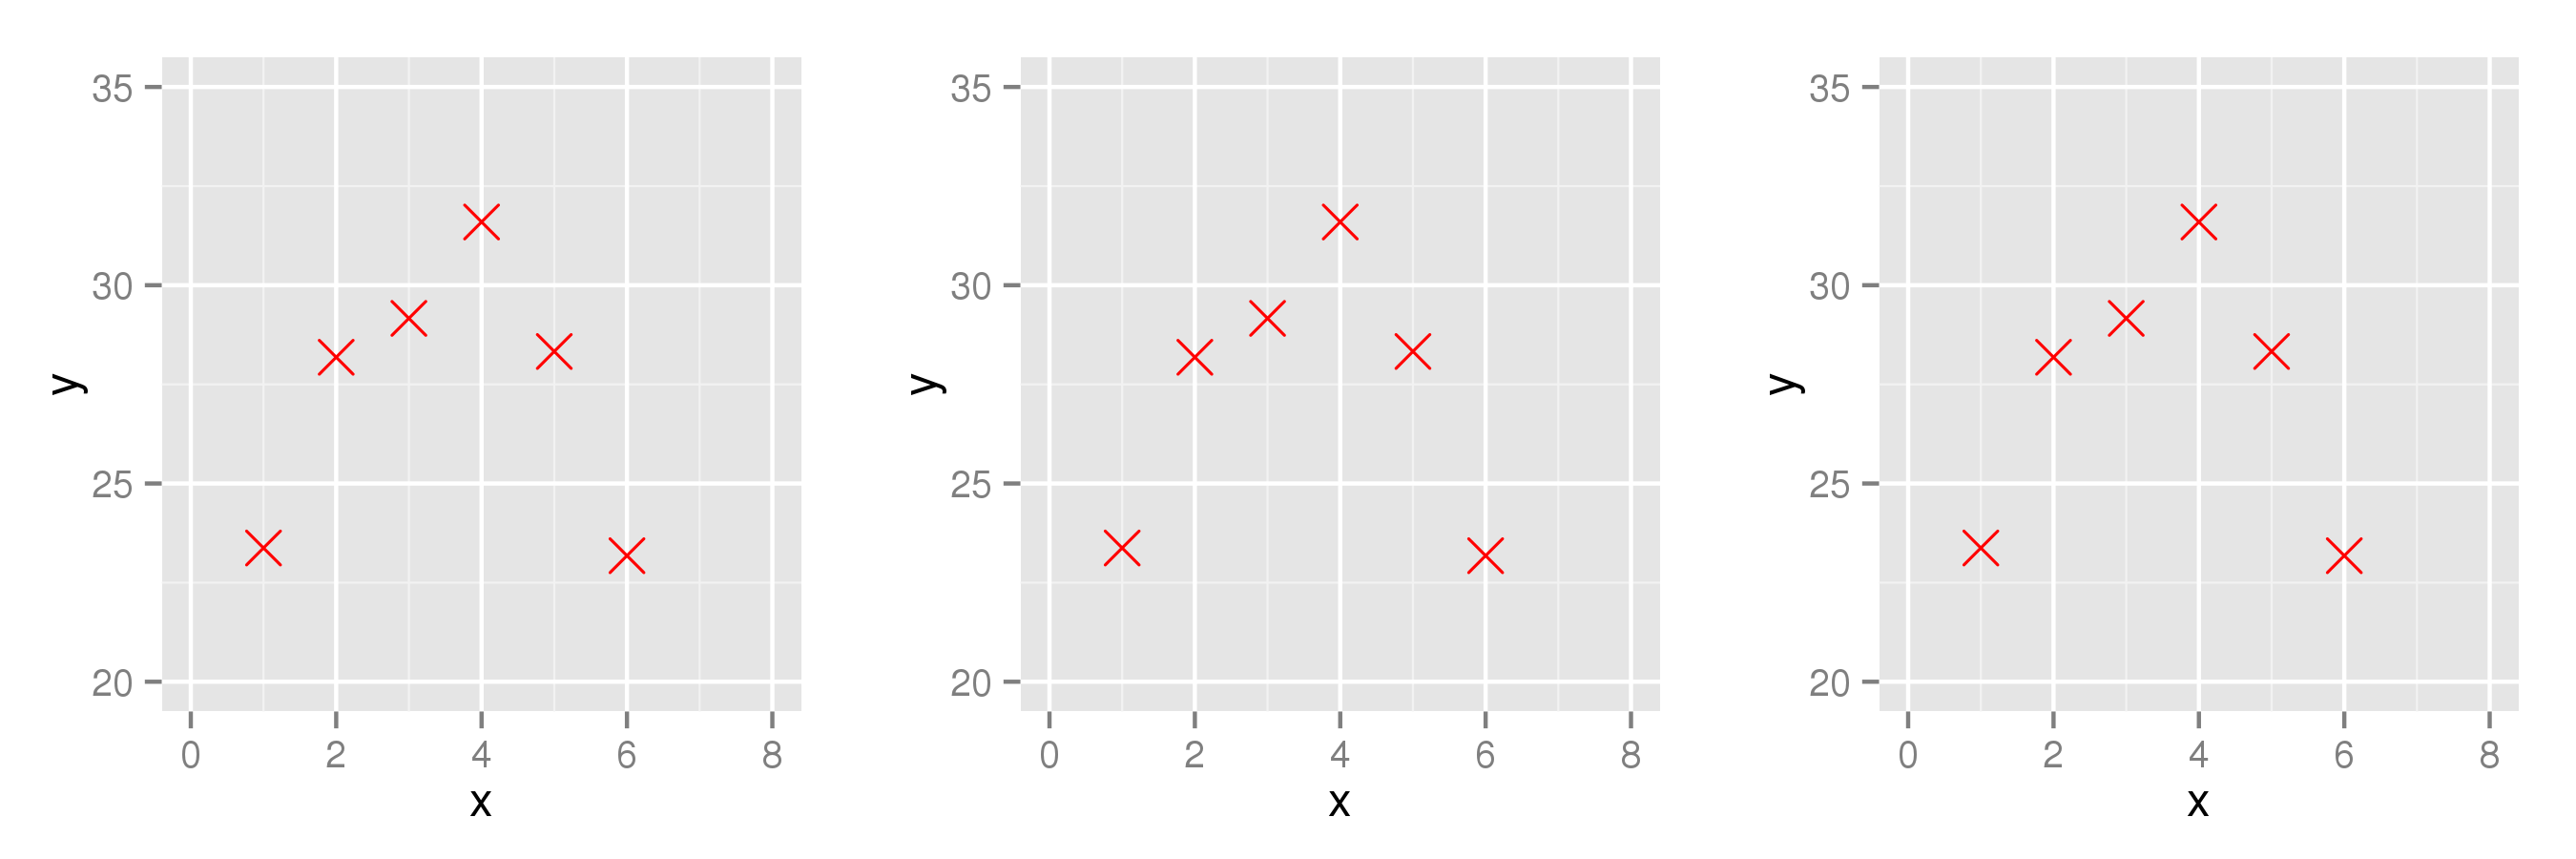
\includegraphics[height=3cm]{xyregularization000.png}
 \end{center}
   \end{overlayarea}
   
 \end{frame}
  \begin{frame}\frametitle{Ejemplo: Ajuste con una característica $x$}
   \begin{overlayarea}{\textwidth}{8cm} 
 \begin{center}
   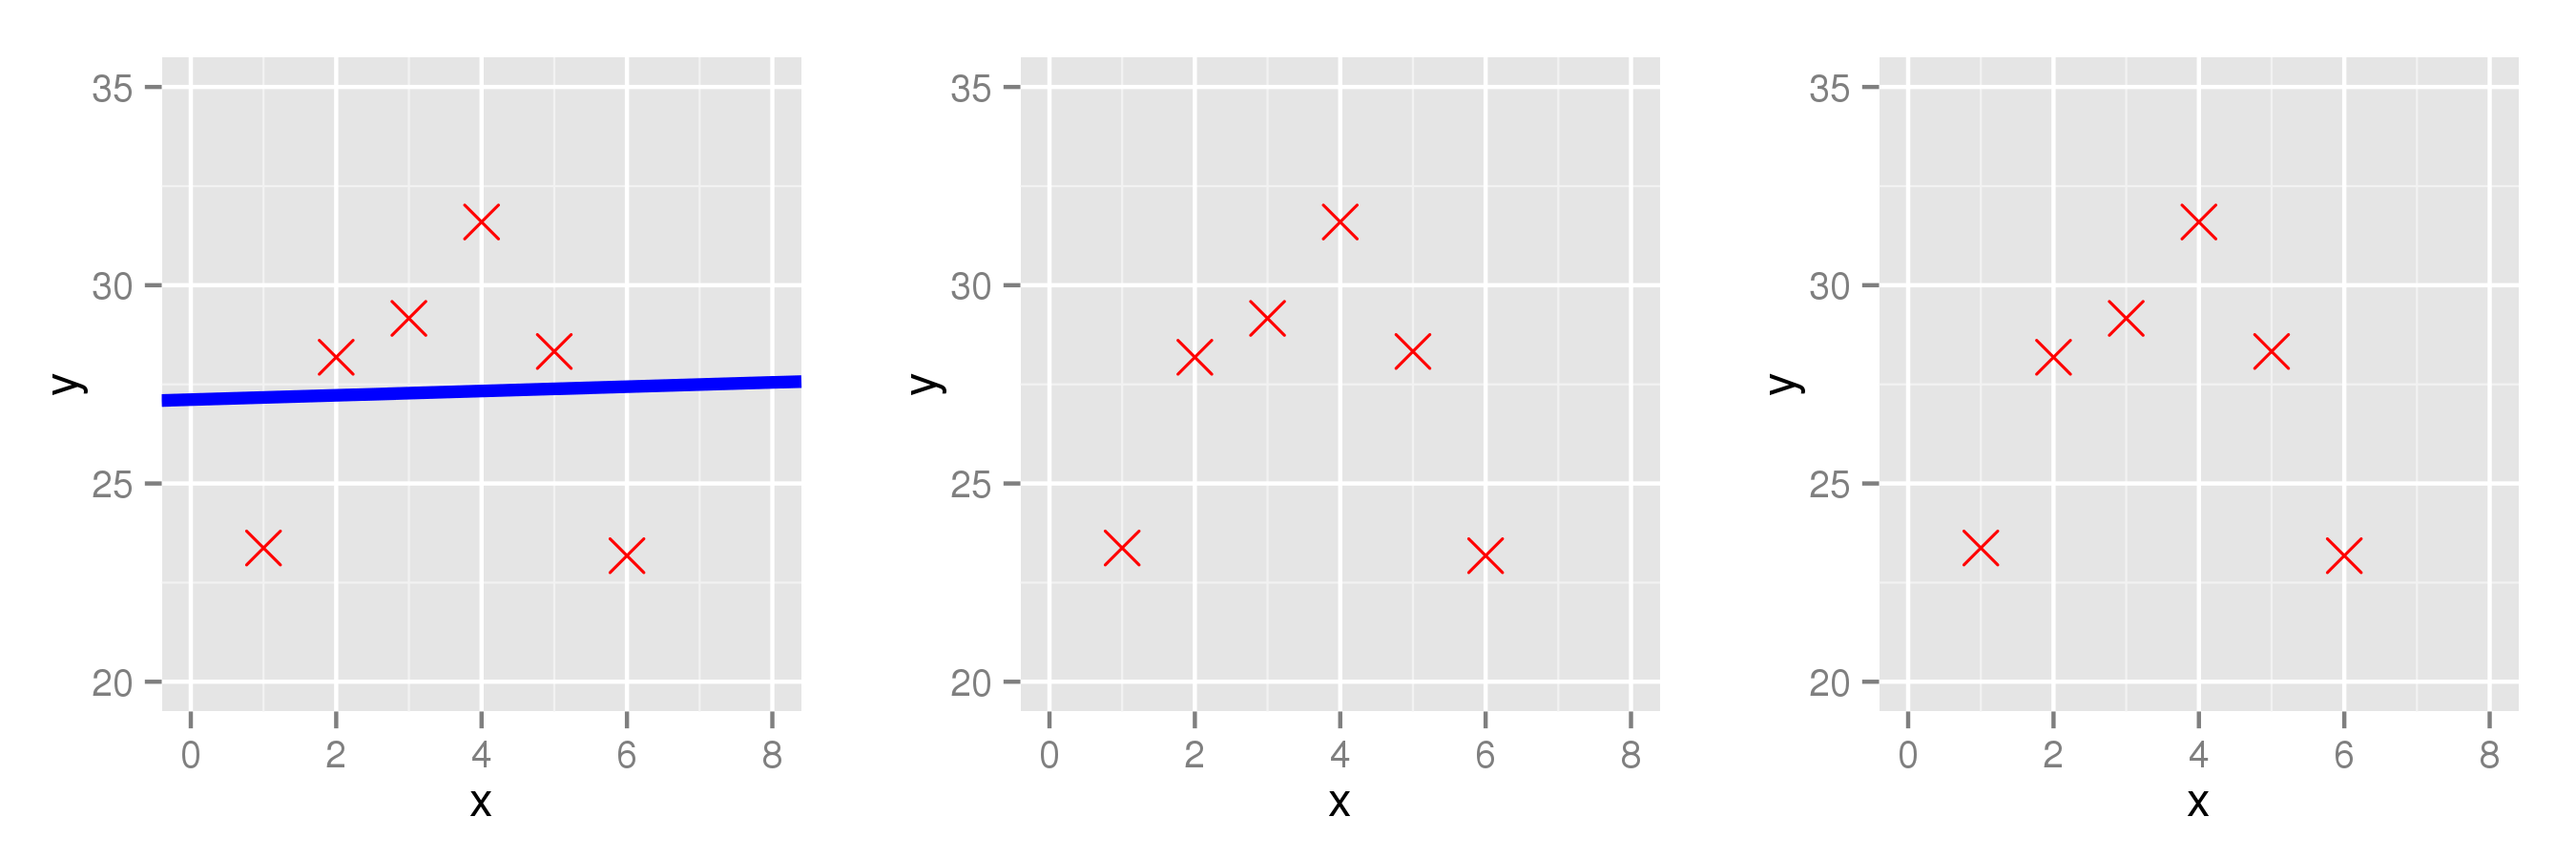
\includegraphics[height=3cm]{xyregularization100.png}
 \end{center}
     \begin{itemize}
 \item Ajuste con una recta: $y=\theta_0+\theta_1x$, mal ajuste ``high bias'' 
 \end{itemize}

   \end{overlayarea}

 \end{frame}
    \begin{frame}\frametitle{Ejemplo: Ajuste con una característica $x$}
   \begin{overlayarea}{\textwidth}{8cm} 
 \begin{center}
   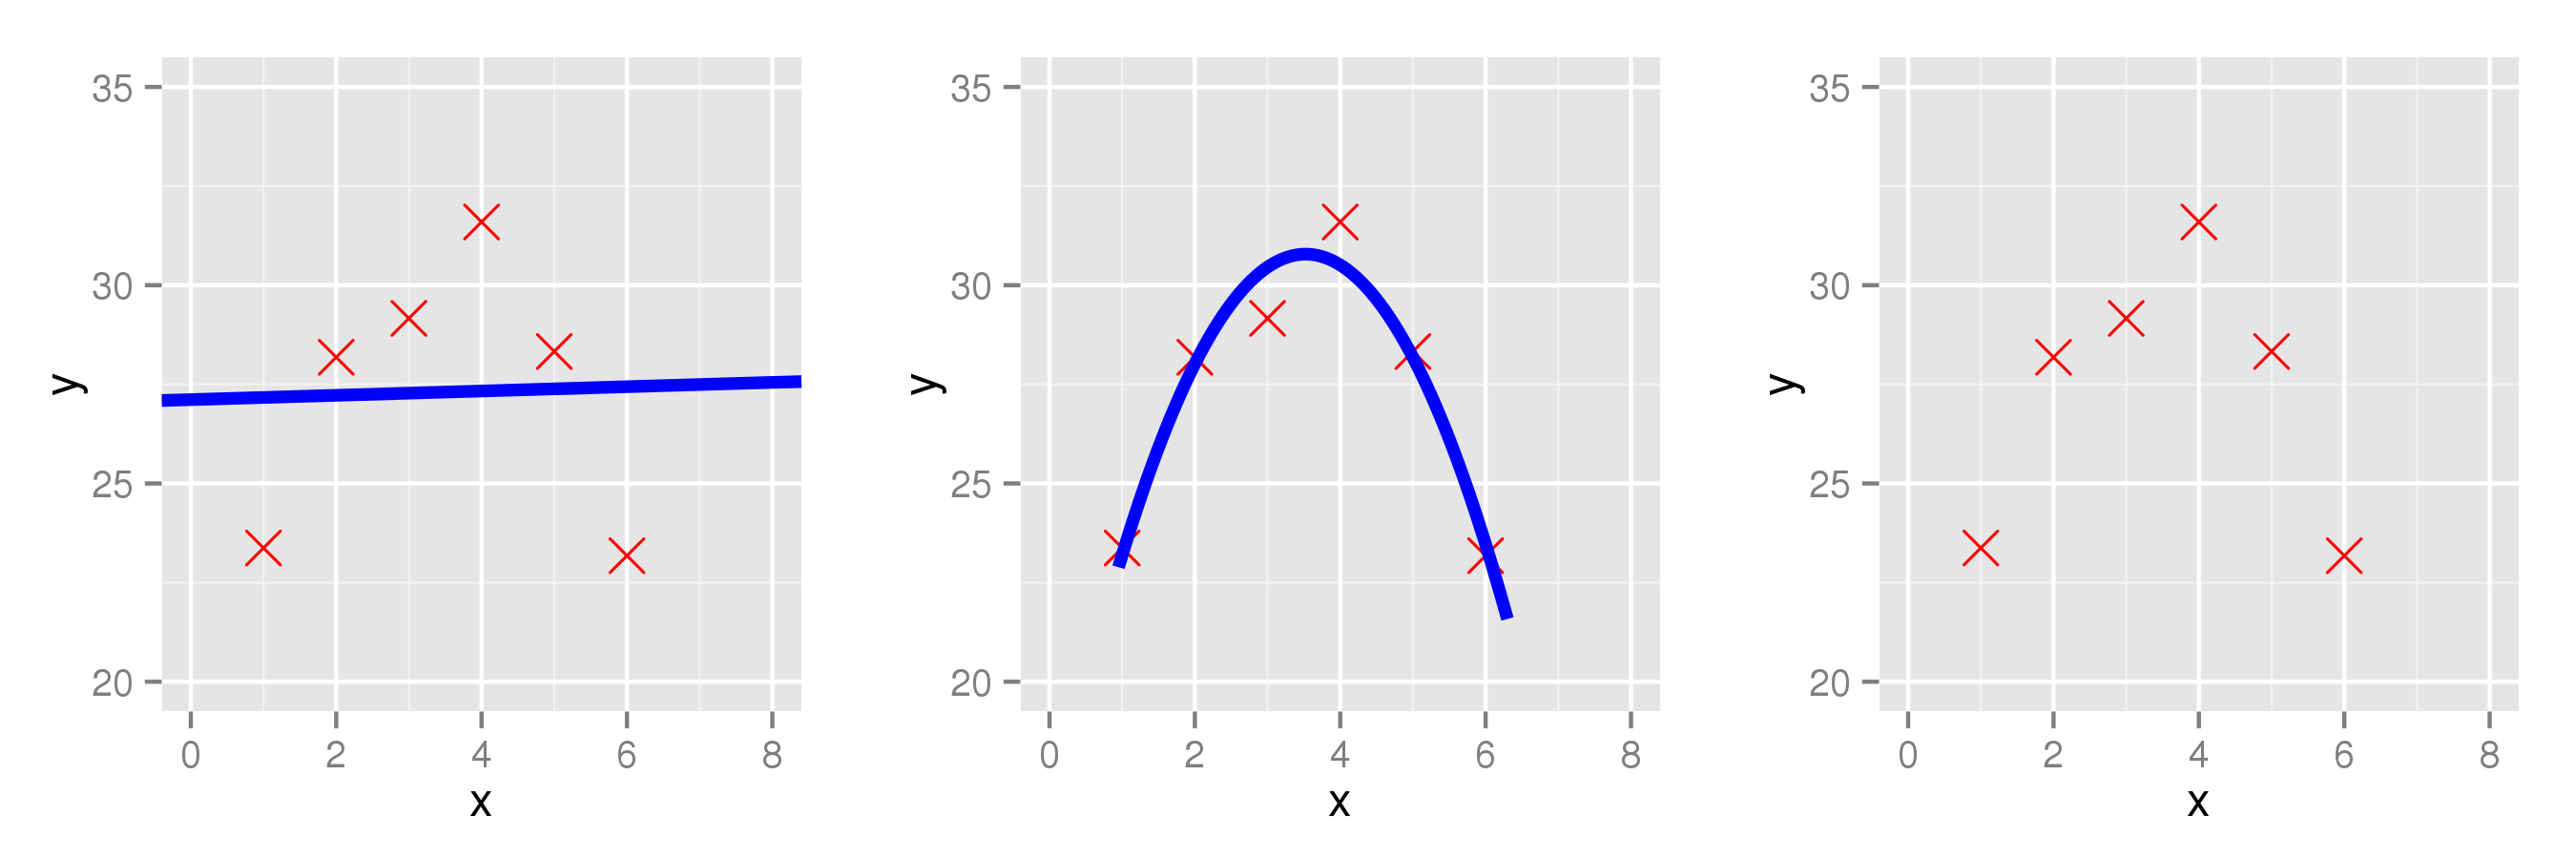
\includegraphics[height=3cm]{xyregularization120.png}
 \end{center}
     \begin{itemize}
 \item Ajuste con una recta: $y=\theta_0+\theta_1x$, mal ajuste ``high bias'' 
    \item Parábola $y=\theta_0+\theta_1x+\theta_2x^2$, ajuste adecuado.
 \end{itemize}

   \end{overlayarea}

 \end{frame}
      \begin{frame}\frametitle{Ejemplo: Ajuste con una característica $x$}
   \begin{overlayarea}{\textwidth}{8cm} 
 \begin{center}
   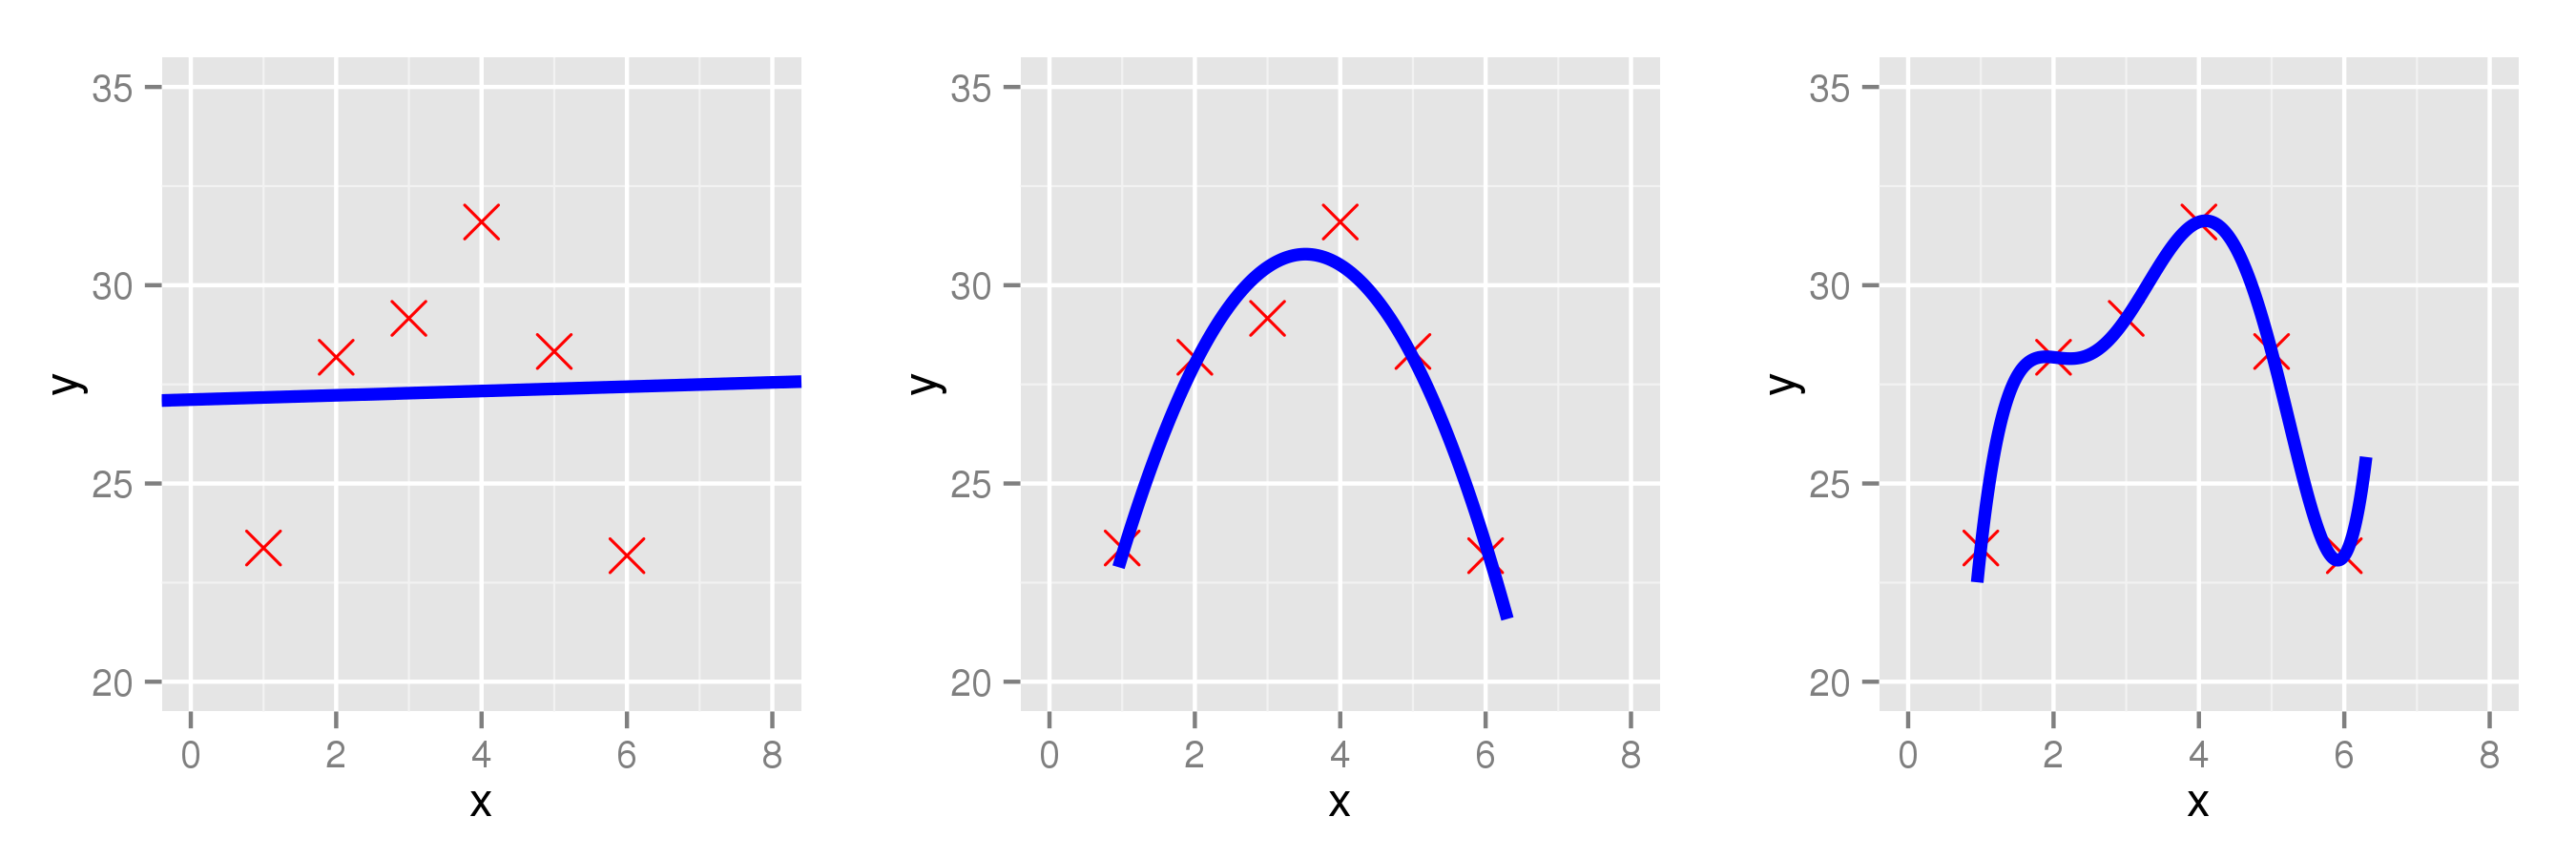
\includegraphics[height=3cm]{xyregularization123.png}
 \end{center}
     \begin{itemize}
 \item Ajuste con una recta: $y=\theta_0+\theta_1x$, mal ajuste. ``High bias.'' 
 \item Parábola $y=\theta_0+\theta_1x+\theta_2x^2$, ajuste adecuado.
 \item Polinomio orden 5: $y=\theta_0+\theta_1x+\ldots+\theta_5x^5$, ajuste  artificialmente bueno... ``High variance.''
 \end{itemize}

   \end{overlayarea}

 \end{frame}
 \begin{frame}\frametitle{Si usamos los modelos para predecir}
      \begin{overlayarea}{\textwidth}{8cm} 
 \begin{center}
   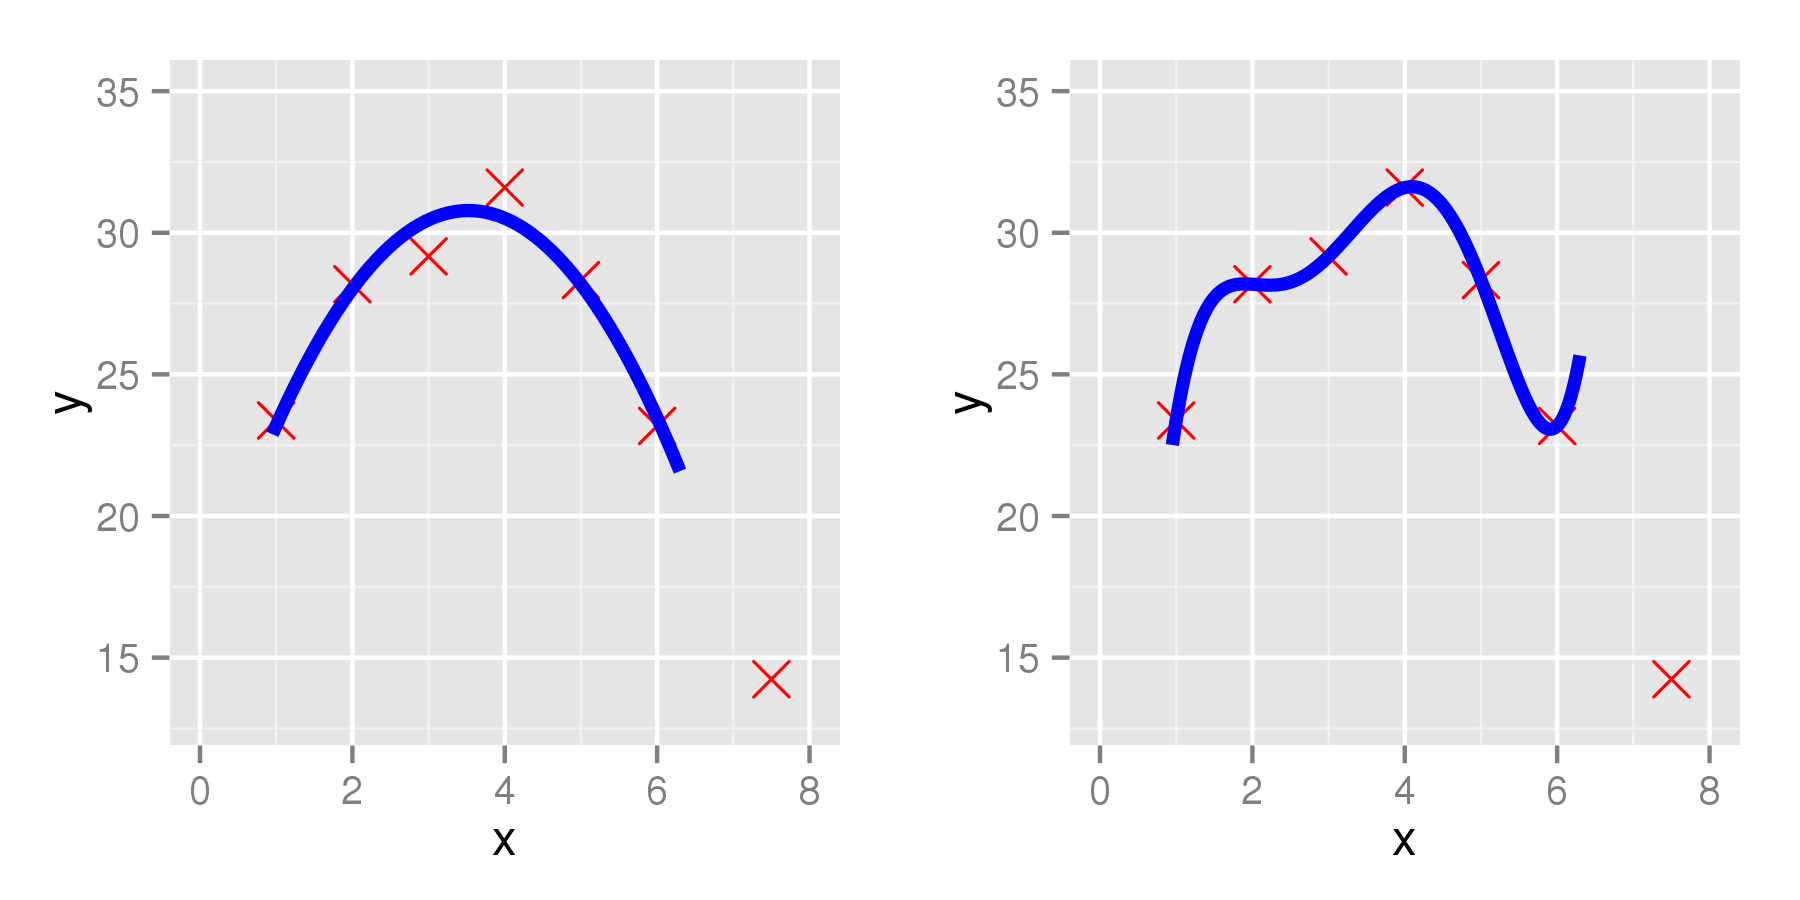
\includegraphics[height=4cm]{xyregularization-prediccion2050.png}
 \end{center}

   \end{overlayarea}

 \end{frame}
  \begin{frame}\frametitle{Si usamos los modelos para predecir}
      \begin{overlayarea}{\textwidth}{8cm} 
 \begin{center}
   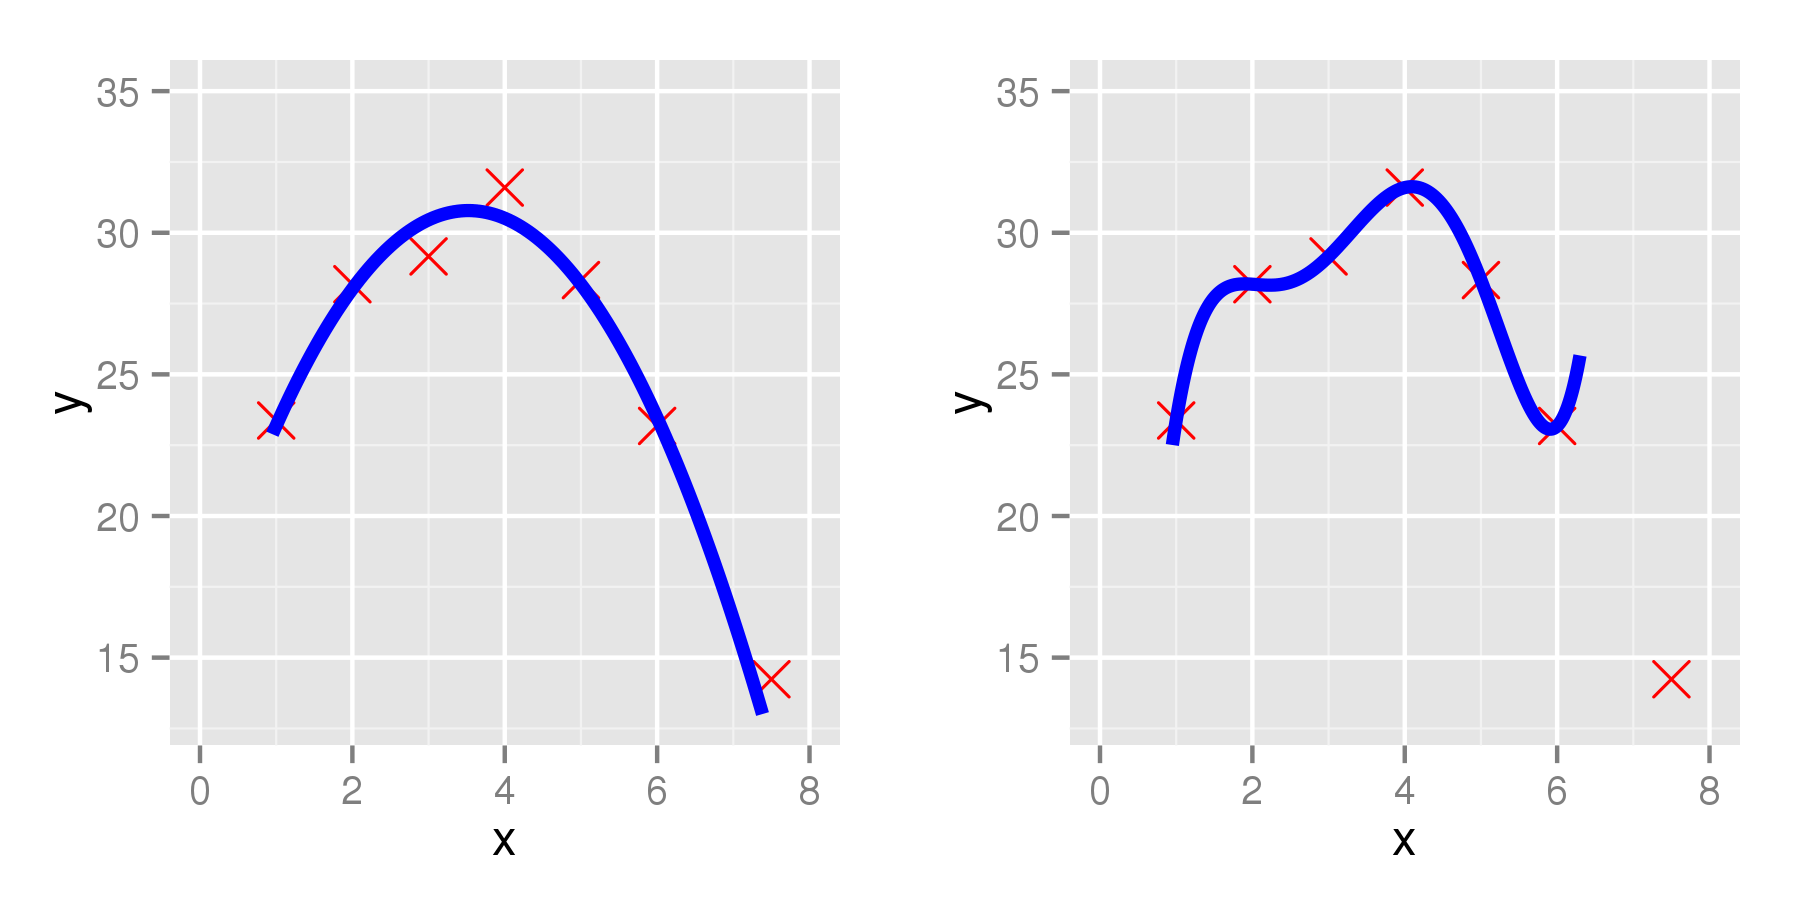
\includegraphics[height=4cm]{xyregularization-prediccion2150.png}
 \end{center}
     \begin{itemize}
 \item Parábola $y=\theta_0+\theta_1x+\theta_2x^2$, predicción correcta.
 \end{itemize}

   \end{overlayarea}

 \end{frame}
   \begin{frame}\frametitle{Si usamos los modelos para predecir}
      \begin{overlayarea}{\textwidth}{8cm} 
 \begin{center}
   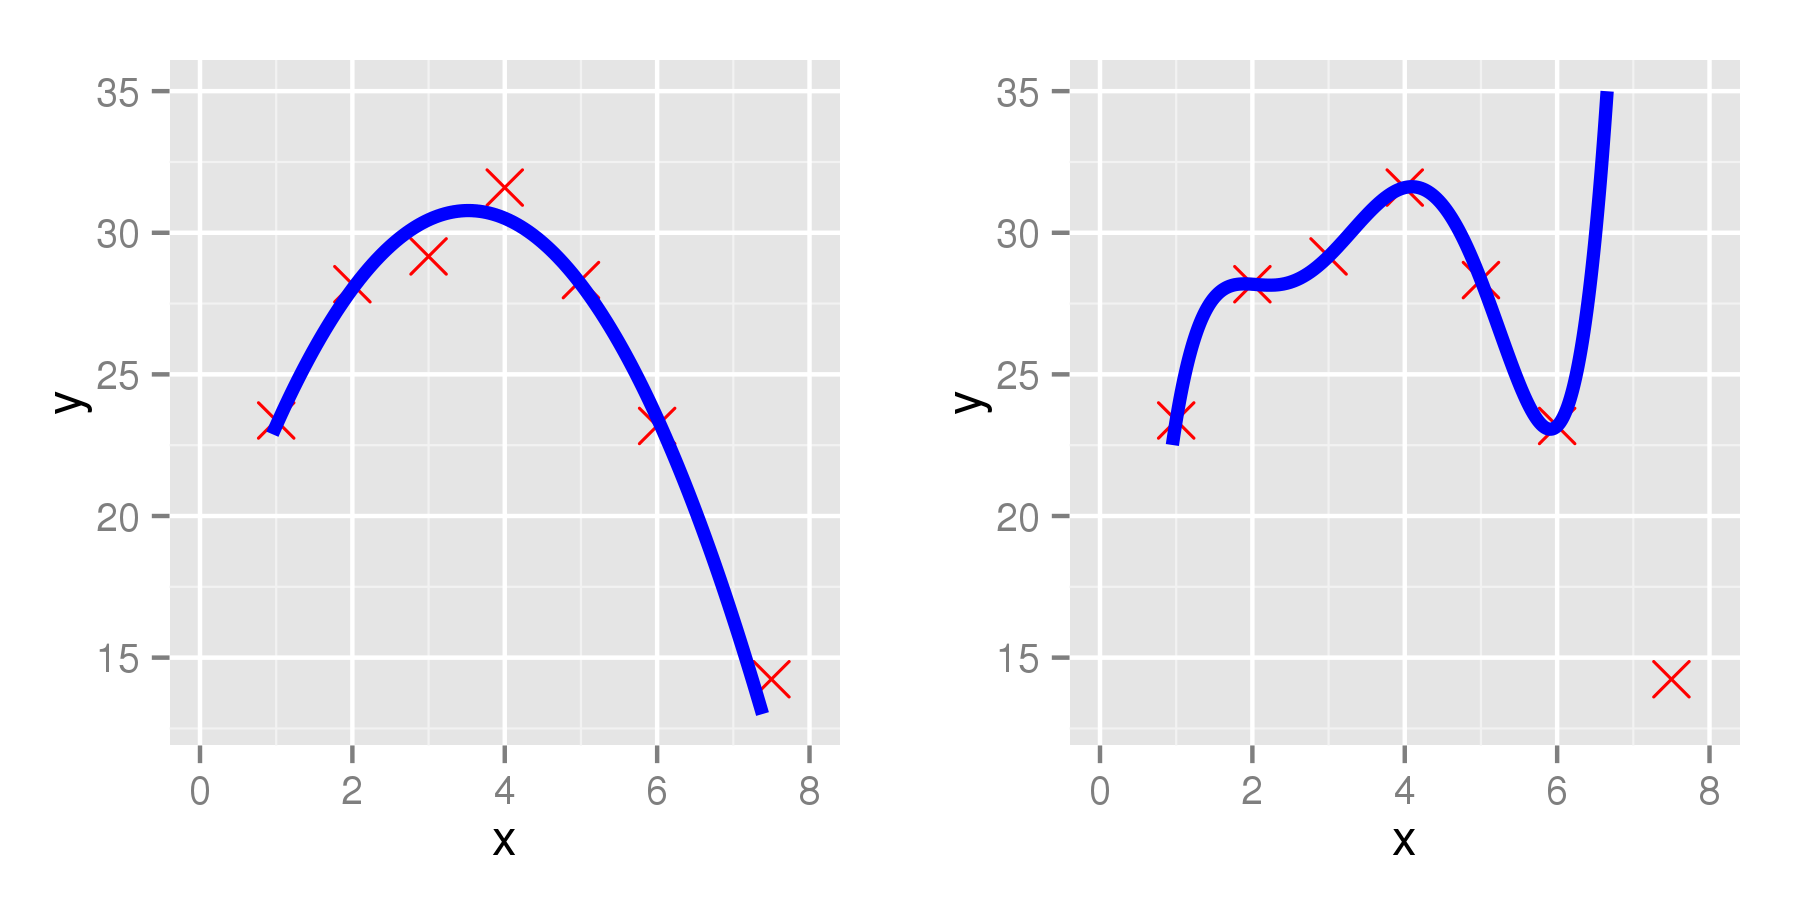
\includegraphics[height=4cm]{xyregularization-prediccion2151.png}
 \end{center}
     \begin{itemize}
 \item Parábola $y=\theta_0+\theta_1x+\theta_2x^2$, predicción correcta.
 \item Polinomio orden 5: $y=\theta_0+\theta_1x+\ldots+\theta_5x^5$, predicción muy mala.
 \end{itemize}

   \end{overlayarea}

 \end{frame}
    \begin{frame}\frametitle{Ejemplo: Clasificación con dos características $x_1$ y $x_2$.}
   \begin{overlayarea}{\textwidth}{8cm} 
 \begin{center}
   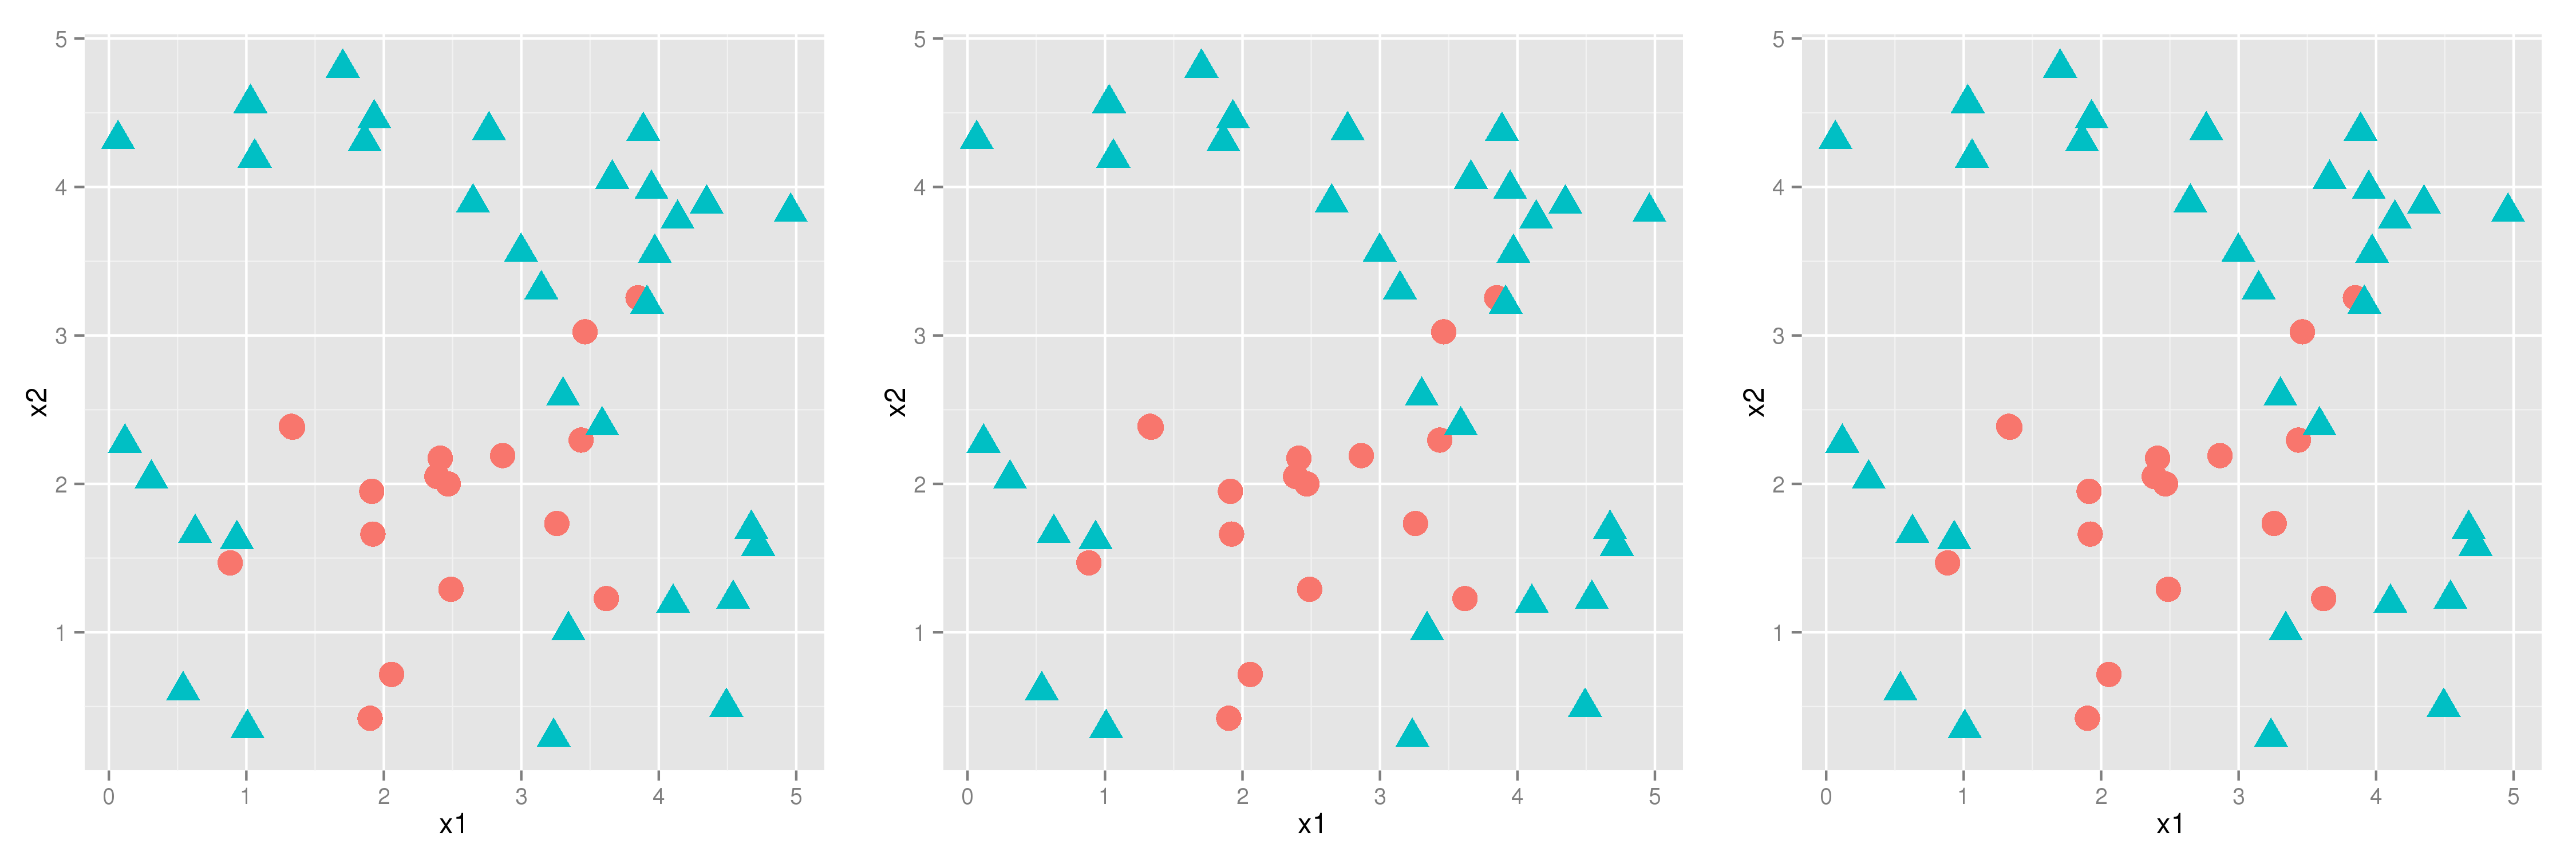
\includegraphics[height=3cm]{decisionboundaries-000.png}
 \end{center}
   \end{overlayarea}
   
 \end{frame}
  \begin{frame}\frametitle{Ejemplo: Clasificación con dos características $x_1$ y $x_2$.}
   \begin{overlayarea}{\textwidth}{8cm} 
 \begin{center}
   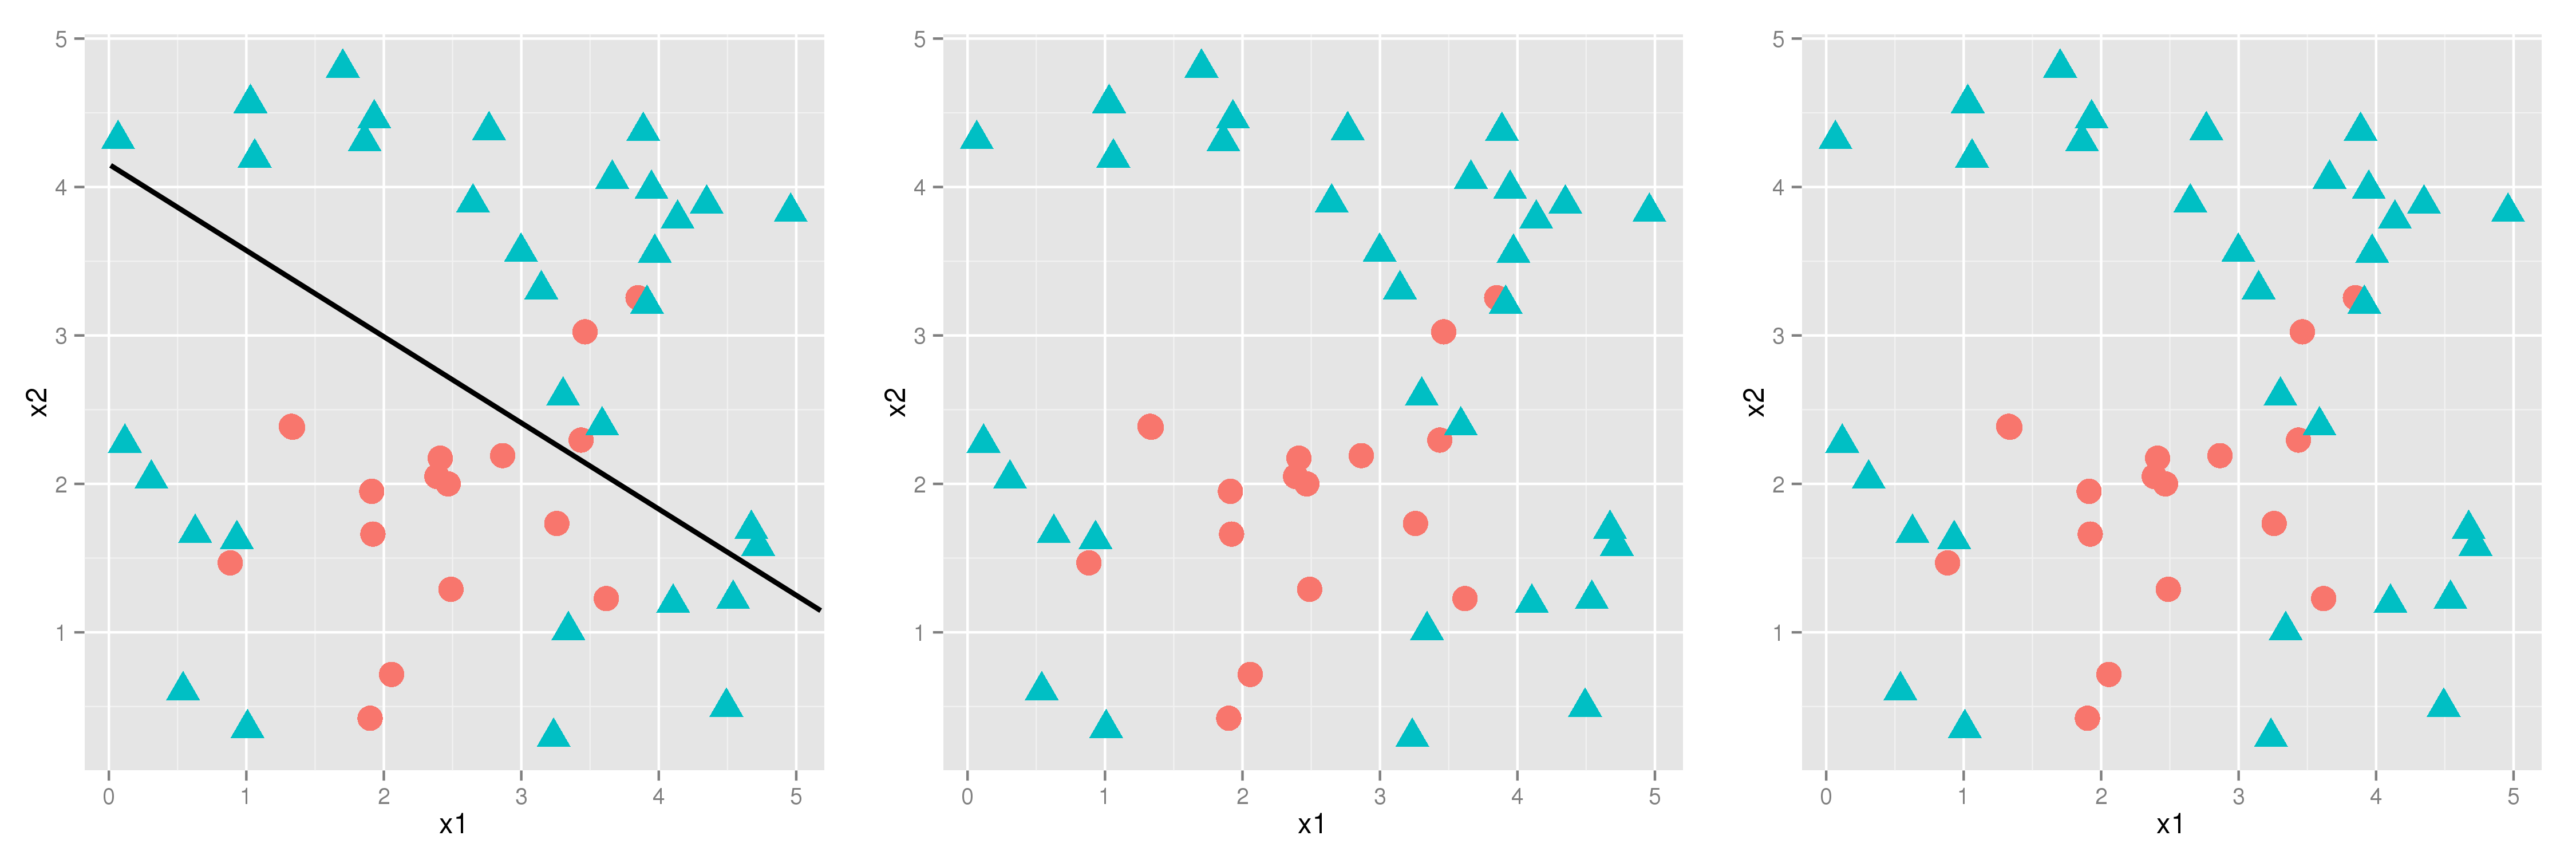
\includegraphics[height=3cm]{decisionboundaries-100.png}
 \end{center}
     \begin{itemize}
 \item Clasificación, frontera es una  recta: $y=g(\theta_0+\theta_1x_1+\theta_2x_2)$.
 \end{itemize}

   \end{overlayarea}

 \end{frame}

    \begin{frame}\frametitle{Ejemplo: Clasificación con dos características $x_1$ y $x_2$.}
   \begin{overlayarea}{\textwidth}{8cm} 
 \begin{center}
   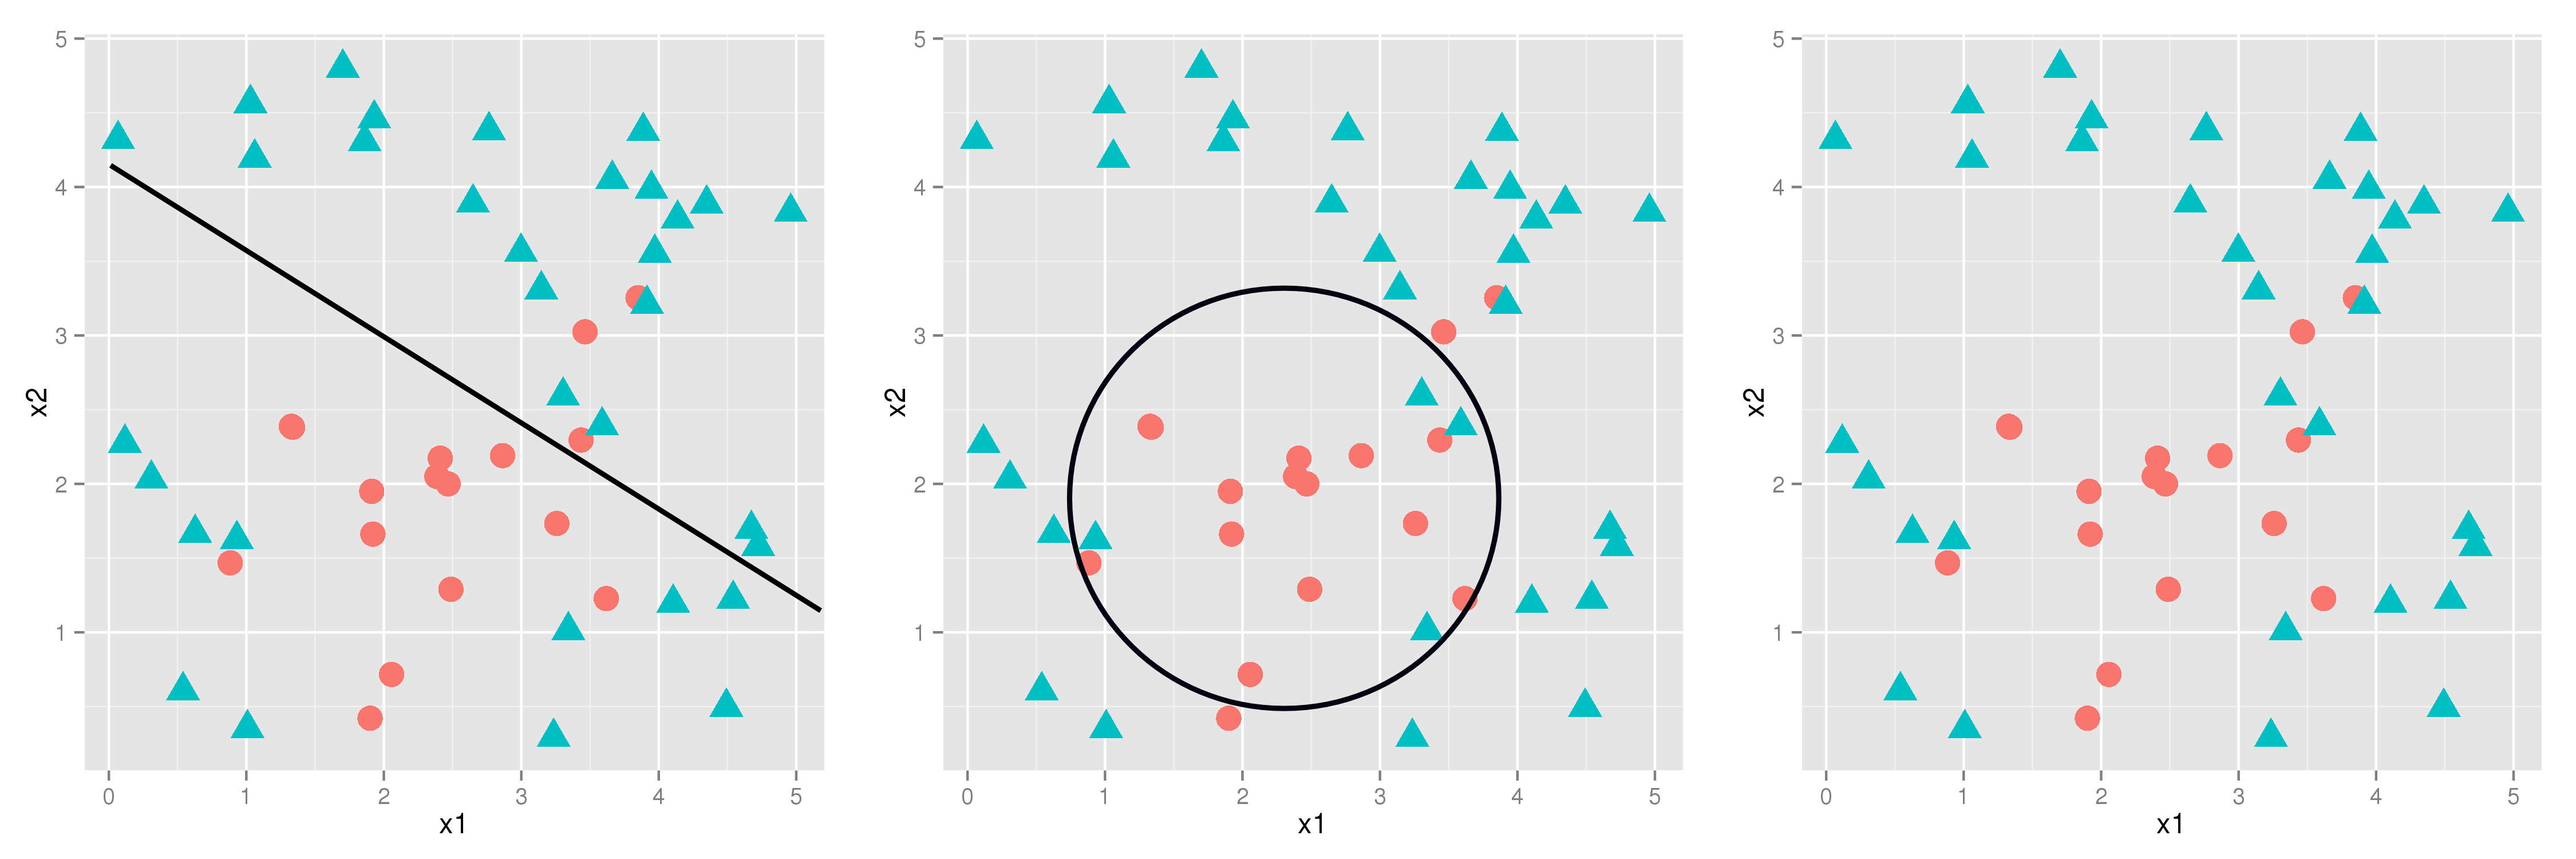
\includegraphics[height=3cm]{decisionboundaries-110.png}
 \end{center}
     \begin{itemize}
 \item Clasificación, frontera es una  recta: $y=g(\theta_0+\theta_1x_1+\theta_2x_2)$.
    \item Clasificación, frontera es un círculo: $y=g(\theta_0+\theta_1x_1+\theta_2x_2+\theta_1x_1^2+\ldots)$.
 \end{itemize}

   \end{overlayarea}

 \end{frame}
      \begin{frame}\frametitle{Ejemplo: Clasificación con dos características $x_1$ y $x_2$.}
   \begin{overlayarea}{\textwidth}{8cm} 
 \begin{center}
   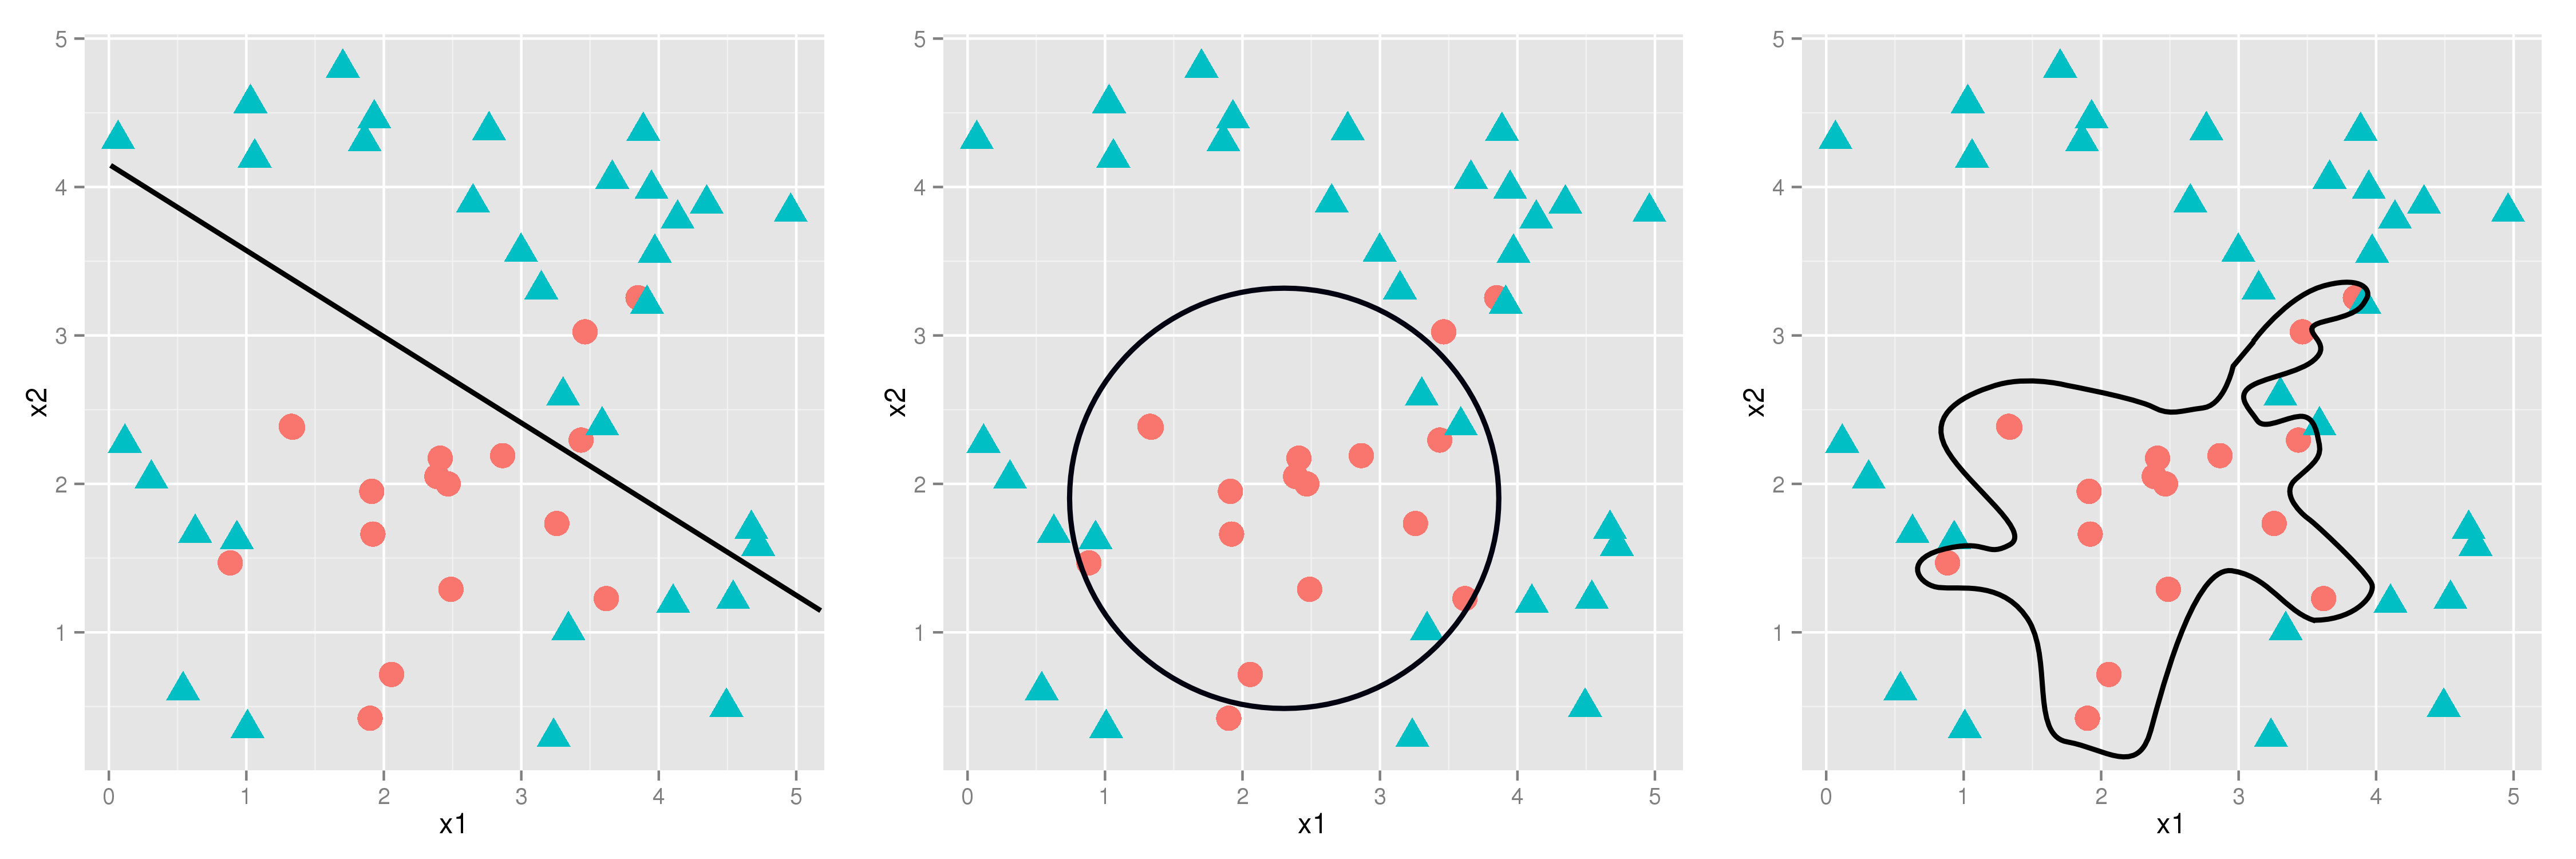
\includegraphics[height=3cm]{decisionboundaries-111.png}
 \end{center}
     \begin{itemize}
 \item Clasificación, frontera es una  recta: $y=g(\theta_0+\theta_1x_1+\theta_2x_2)$.
       \item Clasificación, frontera es un círculo: $y=g(\theta_0+\theta_1x_1+\theta_2x_2+\theta_1x_1^2+\ldots)$.
\item Clasificación, frontera con polinomios orden superior $y=g(\theta_0+\theta_1x_1+\theta_2x_2+\theta_1x_1^2+\ldots+\theta_1x_1^6+\ldots)$.
 \end{itemize}

   \end{overlayarea}

 \end{frame}
 \begin{frame}\frametitle{Para evitar el sobre ajuste (overfitting)}
   \begin{overlayarea}{\textwidth}{8cm} 
     \begin{itemize}
     \item<2-> Podríamos seleccionar manualmente las características que pensamos que pueden servir, sin pasarnos...
     \item<3-> Podemos usar técnicas de selección de modelos: criterios estadísticos de elección de las características más informativas.
     \item<4-> Podemos introducir un término en la función coste que penaliza los ajustes con demasiadas variables...\\ \onslide<5-> Es lo que llamamos la \textcolor{red}{regularización}.
     \end{itemize}

   \end{overlayarea}
   
 \end{frame}

 
 \begin{frame}\frametitle{Modificación de la función coste: regresión lineal}
   \begin{overlayarea}{\textwidth}{8cm} 
     Consideramos la regresión lineal múltiple, la función coste es: 
$$J(\theta)=\frac 1 n\sum_{i=1}^n\left(y_i-f(\theta,x_{i\bullet})\right)^2,$$
     donde $\theta=(\theta_0,\ldots,\theta_k)$ y $x_{i\bullet}$ denota el vector de características para el individuo $i$. 
 \onslide<2->
 \begin{block}{Regularización: primera opción, $l_2$.}
 Añadimos un término: 
 $$J(\theta)=\frac 1
 n\sum_{i=1}^n\left(y_i-f(\theta,x_{i\bullet})\right)^2 +  \frac \lambda {2n}  \sum_{j=1}^{k}\theta_i^2, $$
 donde $\lambda$ es un número positivo que tendremos que fijar.   
 \end{block}
   \end{overlayarea}
 \end{frame}


 \begin{frame}\frametitle{Regularización para regresión lineal}
   \begin{overlayarea}{\textwidth}{8cm} 
      La nueva función coste: 
 $$J(\theta)=\frac 1 n\sum_{i=1}^n\left(y_i-f(\theta,x_{i\bullet})\right)^2 + \frac \lambda {2n} \sum_{j=1}^{k}\theta_i^2, $$

 \begin{itemize}
 \item<2-> \textcolor{red}{Ojo:} el sumatorio $\sum_{j=1}^{k}\theta_i^2$ empieza en $j=1$, no incluye $\theta_0$ (porque corresponde al término constante).
 \item<3-> Si $\lambda$ es grande, para minimizar la función coste, se tenderá hacia una solución donde $\theta_1^2+\cdots+\theta_k^2$ será pequeño, por ejemplo si varios son casi nulos.
 \item<4-> Ajustaremos el valor de $\lambda$, según si queremos penalizar mucho las soluciones con muchos términos significativos o no...
 \end{itemize}

   \end{overlayarea}
   
 \end{frame}

 \begin{frame}\frametitle{Regularización para regresión lineal}
   \begin{overlayarea}{\textwidth}{8cm} 
      La nueva función coste: 
 $$J(\theta)=\frac 1 n\sum_{i=1}^n\left(y_i-f(\theta,x_{i\bullet})\right)^2 +\frac \lambda {2n} \sum_{j=1}^{k}\theta_i^2, $$

 \begin{itemize}
 \item Hablamos de regularización $l_2$, porque el término que se
   añade es proporcional a la norma $l_2$ del vector de parámetros
   $\theta[-1]=(0,\theta_1,\ldots,\theta_k).$,
   $$\lvert\lvert \theta[-1]\rvert\rvert^2 = \sum_{j=1}^{k}\theta_i^2.$$
 \end{itemize}\vspace{-0.5cm}
 \onslide<2->
 \begin{block}{}
   Esta versión de la regresión regularizada se llama \alert{``Ridge
   regression''}.
 \end{block}

   \end{overlayarea}
   
 \end{frame}

       \begin{frame}\frametitle{Función de coste regularizada para la regresión múltiple.}
   \begin{overlayarea}{\textwidth}{8cm} 
   Recordemos las notaciones para la regresión lineal múltiple.\\ Para nuestro conjunto de entrenamiento que consta de $n$ filas, habíamos introducido:
  
$$\mathbf{y}=\left(\begin{array}{l}
y_1\\\vdots\\y_n  
\end{array}\right) \quad\mbox{y la matriz}\quad \mathbf{X}=\left(
\begin{array}{llll}
x_{10}&x_{11}&\cdots&x_{1k}\\
x_{20}&x_{21}&\cdots&x_{2k}\\
\vdots&\vdots&\vdots&\vdots\\
  x_{n0}&x_{n1}&\cdots&x_{nk}\\
\end{array}\right)$$ 
   \end{overlayarea}
   
 \end{frame} 
       \begin{frame}\frametitle{Función de coste regularizada para la regresión lineal}
   \begin{overlayarea}{\textwidth}{8cm} 
   La función de coste regularizada para la regresión lineal
      \begin{center}
\fcolorbox{red}{white}{$\displaystyle J(\theta)=\frac 1
  n\sum_{i=1}^n\left(y_i-x_{i\bullet}^T\theta\right)^2 + \frac \lambda
  {2n}\sum_{j=1}^k \theta_j^2=\frac 1 n\lvert\lvert
  \mathbf{y}-\mathbf{X}\theta\rvert\rvert^2+  \frac \lambda {2n}\lvert\lvert \theta[-1]\rvert\rvert^2,$}
    \end{center}
      donde $\theta[-1]=(0,\theta_1,\ldots,\theta_k).$\\
      \onslide<2-> El gradiente es por lo tanto:
      \begin{center}
\fcolorbox{red}{white}{$ \nabla J(\theta)=\frac 2 n\mathbf{X}^T\cdot \left(\mathbf{X}\theta-y\right)+ \frac \lambda n \theta[-1].  $}
      \end{center}
   \end{overlayarea}
   
 \end{frame}

\begin{frame}[fragile]
   \frametitle{Ridge regression en {\tt scikit-learn}}
   \begin{overlayarea}{\textwidth}{\textheight} 
   Para implementar Ridge regression en {\tt scikit-learn}, se puede
   usar la clase \pyv{Ridge} del súbmodulo \pyv{linear_model}.
   \begin{pyverbatim}
from sklearn.linear_model import Ridge     
\end{pyverbatim}
\medskip

\onslide<2->
A la hora de instanciar nuestro estimador, podemos fijar el valor de
$\lambda$ que multiplica la norma $l_2$, especificando el parámetro
{\tt alpha}.
\begin{pyverbatim}
ridge_reg = Ridge(alpha=1)  
\end{pyverbatim}
\end{overlayarea}   
\end{frame}

 \begin{frame}\frametitle{Regularización: segunda opción, $l_1$.}\vspace{-0.3cm}
   \begin{overlayarea}{\textwidth}{\textheight} 
 \begin{block}{}
 Añadimos un término: 
 $$J(\theta)=\frac 1
 n\sum_{i=1}^n\left(y_i-f(\theta,x_{i\bullet})\right)^2 +  \frac
 \lambda n  \sum_{j=1}^{k}\vert \theta_i\vert, $$
 donde $\lambda$ es un número positivo que tendremos que fijar.   
\end{block}\onslide<2->
\begin{block}{}
   Esta versión de la regresión regularizada se llama \textit{Least Absolute
   Shrinkage and Selection Operator Regression}, i.e. \alert{``Lasso
   regression''}.
 \end{block}
 \onslide<3->
 Una característica importante de la regresión Lasso es que descarta
 completamente las características menos importantes (sus coeficientes
 son 0).
   \end{overlayarea}
 \end{frame}
\begin{frame}[fragile]
   \frametitle{Lasso regression en {\tt scikit-learn}}
   \begin{overlayarea}{\textwidth}{\textheight} 
   Para implementar Lasso regression en {\tt scikit-learn}, se puede
   usar la clase \pyv{Lasso} del súbmodulo \pyv{linear_model}.
   \begin{pyverbatim}
from sklearn.linear_model import Lasso
\end{pyverbatim}

\medskip

\onslide<2->

A la hora de instanciar nuestro estimador, podemos fijar el valor de
$\lambda$ que multiplica la norma $l_1$, especificando el parámetro
{\tt alpha}.
\begin{pyverbatim}
lasso_reg = Lasso(alpha=0.1)  
\end{pyverbatim}
\end{overlayarea}   
\end{frame}

 \begin{frame}\frametitle{Regularización: tercera opción, Elastic net.}
   \begin{overlayarea}{\textwidth}{\textheight}
     Se trata de una combinación de Lasso y de Ridge:
 \begin{block}{}
 Añadimos dos términos: 
 $$J(\theta)=\frac 1
 n\sum_{i=1}^n\left(y_i-f(\theta,x_{i\bullet})\right)^2 +r  \frac
 \lambda n  \sum_{j=1}^{k}\vert \theta_i\vert + (1 - r)\frac {\lambda} {2n}\sum_{j=1}^{k}( \theta_i)^2,      $$
{\scriptsize donde $\lambda$ es un número positivo y $r$ es un número entre 0 y 1 que tendremos que fijar.   }
\end{block}\onslide<2-> \scriptsize
\begin{block}{Recomendación}
  \begin{itemize}
  \item    Cuando tenemos bastantes características, es buena idea usar una
   regresión regularizada. 
 \item Si sospechamos que hay varias
   características que no son relevantes, entonces se recomienda usar
   Lasso o Elastic Net.
 \item Elastic Net is preferible cuando hay más características que
   individuos en el conjunto de aprendizaje o cuando están las
   características muy correlacionadas.
  \end{itemize}

 \end{block}

   \end{overlayarea}
 \end{frame}
\begin{frame}[fragile]
   \frametitle{Elastic net regression en {\tt scikit-learn}}
   \begin{overlayarea}{\textwidth}{\textheight} 
   Para implementar Elastic Net {\tt scikit-learn}, se puede
   usar la clase \pyv{ElasticNet} del súbmodulo \pyv{linear_model}.
   \begin{pyverbatim}
from sklearn.linear_model import ElasticNet
\end{pyverbatim}
\medskip

\onslide<2->
A la hora de instanciar nuestro estimador, podemos fijar el valor de
$\lambda$ que multiplica las normas $l_1$ y $l_2$, especificando el parámetro
{\tt alpha}, y el valor de $r$ que indica el peso de la norma $l_1$
frente  a la norma $l_2$, especificando el parámetro {\tt l1\_ratio}
\begin{pyverbatim}
elastic_net = ElasticNet(alpha=0.1, l1_ratio=0.5)  
\end{pyverbatim}
\end{overlayarea}   
\end{frame}

\begin{frame}\frametitle{Función de coste regularizada para la regresión logística}
Vimos en las transparencias de la clase anterior que, para la regresión logística, la función de coste sin regularizar era:
    $$J(\theta)=- \frac 1 n\sum_{i=1}^n \left\{y_i\log(h_\theta(x_{i\bullet}))+(1-y_i)\log(1-h_\theta(x_{i\bullet}))\right\},$$
donde $h_\theta(x_{i\bullet})=g(x_{i\bullet}\theta)=1/(1+exp(-x_{i\bullet}\theta)).$
\end{frame}

    \begin{frame}\frametitle{Función de coste regularizada para la regresión logística}
Además el gradiente es.
$$    \nabla_\theta J(\theta)= \frac 1 n\sum_{i=1}^n \left\{x_{i\bullet}\cdot (h_\theta(x_{i\bullet})-y_i)\right\}.$$
Si usamos la matriz de diseño $\mathbf{X}$,   obtuvimos  en forma compacta:
$$    \nabla_\theta J(\theta)=\frac 1  n \mathbf{X}^T\cdot\left(\mathbf{H}_\theta-y\right).$$
 donde $\mathbf{H}$ denota el vector columna:
$$\mathbf{H}_\theta=\left(
\begin{array}{l}
  h_\theta(x_{1\bullet})\\
  h_\theta(x_{2\bullet})\\
  \vdots\\
  h_\theta(x_{n\bullet})\\
\end{array}\right)$$

\end{frame}

              \begin{frame}\frametitle{Función de coste regularizada para la regresión logística}
   \begin{overlayarea}{\textwidth}{8cm} 
   Podemos regularizar la función de coste para la regresión lógistica
   igual que lo hicimos para la regresión lineal.\footnotesize
   \onslide<2->
   \begin{itemize}
   \item Podemos usar la regularización $l_2$:
   \end{itemize}
   \begin{center}
\fcolorbox{red}{white}{$\displaystyle J(\theta)=- \frac 1 n\sum_{i=1}^n \left\{y_i\log(h_\theta(x_{i\bullet}))+(1-y_i)\log(1-h_\theta(x_{i\bullet}))\right\}+\frac \lambda {2n}\sum_{j=1}^k \theta_j^2$}
\end{center} \onslide<3->
\begin{itemize}
\item o la regularización $l_1$
\end{itemize}
\begin{center}
\fcolorbox{red}{white}{$\displaystyle J(\theta)=- \frac 1 n\sum_{i=1}^n \left\{y_i\log(h_\theta(x_{i\bullet}))+(1-y_i)\log(1-h_\theta(x_{i\bullet}))\right\}+\frac \lambda n\sum_{j=1}^k \vert\theta_j\vert$}
\end{center}
\begin{itemize}
\item<4-> o su combinación en Elastic net.
\end{itemize}
 
\end{overlayarea}
   
\end{frame}

\begin{frame}[fragile]
   \frametitle{Regresión logística en {\tt scikit-learn}}
   \begin{overlayarea}{\textwidth}{\textheight} 
   Ya vimos que para implementar la regresión logística en {\tt scikit-learn}, se puede
   usar la clase \pyv{LogisticRegression} del súbmodulo \pyv{linear_model}.
   \begin{pyverbatim}
from sklearn.linear_model import LogisticRegression
\end{pyverbatim}
\medskip


\begin{itemize}
\item<2-> \pyv{LogisticRegression} admite el parametro {\tt penalty} que puede
tomar el valor \pyv{'l2', 'l1', 'elasticnet'} o \pyv{'none'}.
\item<3-> En lugar de implementar el parámetro \pyv{alpha}, usa el parámetro
  \pyv{C} que es la inversa de $\lambda$ (\pyv{alpha}). 
\item<4-> Por defecto, \pyv{LogisticRegression} usa la regularización
  \pyv{'l2'} con \pyv{C=1}!
\item<5-> También admite el parámetro \pyv{l1_ratio} si \pyv{penalty='elasticnet'}.
\end{itemize}
\end{overlayarea}   
\end{frame}

\end{document}
